\lhead{\emph{Multiresolution Imaging}}
\chapter{Multiresolution Imaging}
\label{ch:imaging}

Imaging applications benefit greatly from multiresolution representations, which allow hierarchical decomposition of an image into different levels of detail. This hierarchical structure mirrors models of human visual perception, such as Marr's vision theory \citep{marr82}, where the visual cortex processes information from low to high spatial frequencies. These models are foundational for tasks in computer vision and graphics, such as compression, analysis, and rendering.


In this chapter, we explore the role of multiresolution techniques in imaging applications and present our proposed MR-Net architecture as a modern alternative to traditional methods. The following sections, based on \citet{paz2022} and \citet{paz2023mr}, detail the implementation and experimentation of MR-Net across various imaging tasks, such as multiresolution encoding, texture magnification and minification, and antialiasing.

Additionally, we provide comprehensive experimental evaluations, comparing MR-Net to existing methods such as SIREN \citep{sitzmann2019siren} and BACON \citep{bacon2021}. Through these comparisons, we illustrate how MR-Net can offer more efficient representations with fewer parameters, all while maintaining or surpassing the performance of traditional approaches. Moreover, we examine the differences between the various MR-Net subclasses, namely S-Net, L-Net, and M-Net.

Finally, the chapter addresses the current limitations of MR-Net and outlines potential future directions. While the architecture presents clear advantages in terms of flexibility and performance, some challenges remain in optimizing frequency initialization and further reducing storage complexity.

% This chapter builds on these foundations, demonstrating the use of our MR-Net architecture for imaging applications. Unlike traditional wavelet or Fourier-based approaches, MR-Net leverages sinusoidal activations to control frequency generation during training, providing detail control across resolutions.  

% We also compare our proposal with previous works, and we discuss differences between MR-Net subclasses and some current limitations of our approach.





% Unlike classical approaches that rely on Fourier or wavelet transforms, MR-Net employs sinusoidal activation functions, allowing for more flexible and precise control over frequency generation during training. This capability enables MR-Net to decompose signals across multiple scales and adaptively balance the resolution and detail representation in a way that reflects the underlying frequency content of the image.

% Through this work, we aim to demonstrate that MR-Net is not just an alternative to traditional multiresolution techniques but a powerful and adaptive framework for modern image processing tasks, with potential implications for a wide range of applications in computer vision and beyond.


\section{Related Works}

The field of multiresolution imaging has a rich history, with methods that go from classical signal processing techniques to more recent neural network-based approaches. Understanding the evolution of these methods provides a context for the contributions of MR-Net.

Traditional multiresolution methods, based on the Laplacian pyramid \citep{burt1987laplacian}, have been central in image compression by facilitating progressive data reduction. These methods focus on identifying and eliminating high-frequency components that contribute minimally to perceptual quality, while preserving essential low-frequency features. By efficiently discarding redundant information, they achieve significant data reduction while maintaining perceptual image integrity. Additionally, in rendering, multiresolution representations inherently support antialiasing, which has traditionally been implemented using image pyramids in methods like Mipmapping \citep{mipmap83}. Texture synthesis also benefits from these techniques, as multiresolution approaches also aid in the creation of visual patterns from exemplar images \citep{thies19}.


Historically, multiresolution representations for images have been rooted in signal processing techniques derived from the Fourier theory \citep{bracewell1986fourier}. The Discrete Cosine Transform (DCT) \citep{dct-og} became particularly useful in image compression, as it enabled efficient analysis of frequency content, prioritizing coefficients most relevant to perceptual quality. The wavelet transform, introduced by \citet{mallat1989theory}, later emerged as a powerful alternative, enabling a multiscale representation of images that could capture both frequency and spatial information at various levels of detail. This innovation led to the first generation of wavelet-based image codecs \citep{antonini1992image} and, subsequently, higher compression rates through more advanced wavelet-based coding methods \citep{mallat-2gen}.

A key advantage of both wavelet and Fourier-based approaches lies in their ability to control and interpret the frequencies present in a signal, which is critical for avoiding artifacts like aliasing. Sinusoidal functions, fundamental to Fourier analysis, enable precise frequency decomposition and control, what emphasize their importance in multiresolution theory. These principles are extended in modern neural network architectures, including the one introduced in this dissertation.

In recent years, coordinate-based neural networks have emerged as powerful tools for learning and representing continuous signals in computer vision and graphics applications. Notable examples include Occupancy Networks \citep{occupancy_networks}, DeepSDF \citep{park2019deepsdf}, NeRF \citep{2020nerf}, and SIREN \citep{sitzmann2019siren}. While some of these methods acknowledge the spectral bias of MLPs and use sinusoidal functions to achieve better results, they lack an explicit, principled connection to frequency-based signal representations or level-of-detail decomposition. MipNeRF \citep{barron2022mipnerf360} introduced a form of multiscale decomposition to improve the efficiency of NeRF rendering, focusing on anti-aliasing and speeding up view synthesis. However, they do not explicitly focus on frequency decomposition, but rather on spatial antialiasing via its multiscale frustum-based sampling, and they do not provide a solution for general signals representation.

% The introduction of Multiplicative Filter Networks (MFNs) \citep{fathony2020multiplicative} marked a significant step forward by directly encoding signals as a sum of frequency components. These architectures, built on sinusoidal activations, provide a more interpretable relationship between neural network parameters and the frequency content of the signals they model. \citet{bacon2021} extended this concept with BACON, building a neural architecture capable of encoding signals across multiple scales. However, as discussed in Chapter \ref{chap:mr_snn}, Bacon's approach relies on truncating the frequency spectrum at predefined levels, which introduces artifacts such as ringing at specific stages of detail. 

\citet{fathony2020multiplicative} introduced the Multiplicative Filter Network (MFN), an architecture based on sinusoidal functions that can be analytically understood as a sum of frequencies. Building on this concept, \citet{bacon2021} developed BACON, an extension of MFN designed to encode signals across multiple scales. However, as discussed in Chapter \ref{chap:mr_snn}, their approach to multiresolution representation relies on truncating the frequency spectrum at predefined values, which leads to ringing artifacts at certain levels of detail. We will demonstrate in Section \ref{sec:comparison} that MR-Net offers a more efficient representation of image spectra, avoiding these artifacts while using fewer parameters than BACON's architecture.


\section{Multiresolution Image Representation}
\label{s:img}


In the following experiments, we employ the M-Net subclass of our architecture, utilizing a level of detail scheme based on the Gaussian Pyramid in all examples. The image pyramid follows a dyadic structure, with resolutions scaling as \( 2^j \). The pyramid is constructed by filtering the image with a Gaussian kernel followed by downsampling (decimation) to achieve progressively coarser representations.

We designed the MR-Module through empirical analysis of the network's capacity to represent typical photographic images. Each stage of the network, except the last one, comprises 96 neurons across all layers in the first, hidden, and output blocks. The last stage is wider, with 256 neurons per layer. The hidden block at each stage contains only one layer. This compact configuration is chosen to balance expressivity and computational efficiency.

For the first stage, we define the base resolution of the input image as \( 2^3 = 8 \) pixels. The number of stages in the network is determined by the maximum resolution of the target image. Unless stated otherwise, the images used in our experiments have a resolution of \(512 \times 512\), resulting in a pyramid consisting of seven resolution levels: 8, 16, 32, 64, 128, 256, and 512. Consequently, the network comprises seven stages, with each stage tasked with refining the image at the corresponding level of detail.

We train the network using an adaptive scheme with the following hyperparameters: the loss function is the Mean Squared Error (MSE), with a convergence threshold of \(0.001\) (i.e., training for a given stage halts when the loss change between epochs is less than \(0.001\)). The maximum number of epochs per stage is set to 300, with each epoch processing all pixels exactly once. The mini-batch size is fixed at 65,536 to fit within the available GPU memory. The network is trained using the Adam optimizer with a learning rate of \(1 \times 10^{-4}\).

The network initialization follows the scheme outlined in Section~\ref{sec:frequency-initialization}, where frequency bands are selected in alignment with the Gaussian/Laplacian pyramid LoD scheme described in Section~\ref{s:lod}. Specifically, \red{the weights of the first layer in each stage are initialized to match the frequency range of the corresponding resolution level}: \(\omega_0\) is uniformly distributed as \( \mathcal{U}(-B_i, B_i)\), where \( B_i = [4, 8, 16, 32, 64, 128, 256]_{i=1}^7 \) for a seven-stage network. For all stages, the weights of the hidden layers are initialized with \(\omega_h = 30\).


\subsection{Level of Detail Example}
\label{ss:LOD}

To illustrate the multiresolution capabilities of the network, we now present an experiment using the "Cameraman" image, a standard benchmark in image processing and used in related works such as \citet{sitzmann2019siren}. The image is a monochrome photograph with a resolution of \(512 \times 512\) pixels.

Figure~\ref{f:lod} shows the reconstructed image at resolution levels 1, 3, 5, and 7, each corresponding to different stages of the network, along with their respective Fourier spectra. These reconstructions demonstrate how the network progressively captures increasing levels of detail as the resolution increases.

\begin{figure}[!ht]
\centering
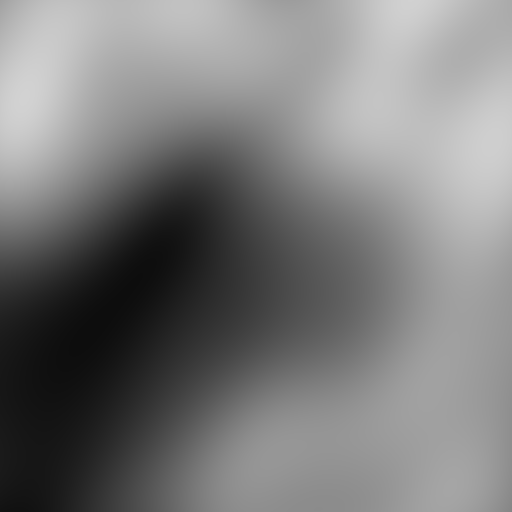
\includegraphics[width=0.22\linewidth]{img/ch5/1-cameraman.png}

\includegraphics[width=0.22\linewidth]{img/ch5/3-cameraman.png}
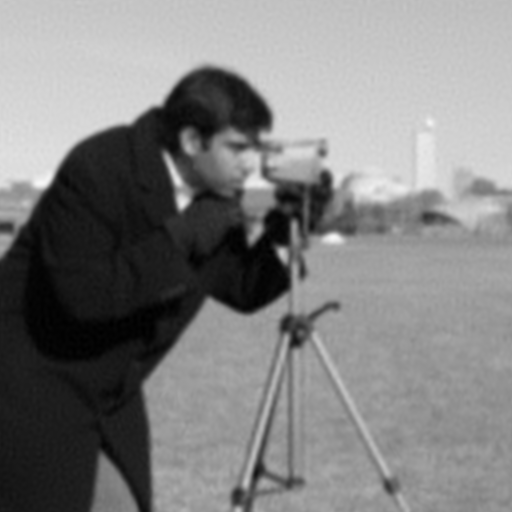
\includegraphics[width=0.22\linewidth]{img/ch5/5-cameraman.png}
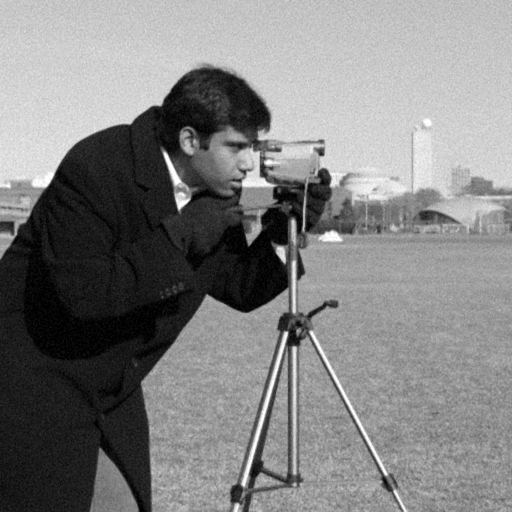
\includegraphics[width=0.22\linewidth]{img/ch5/7-cameraman.png} \\


\includegraphics[width=0.22\linewidth]{img/ch5/1-fft.png}
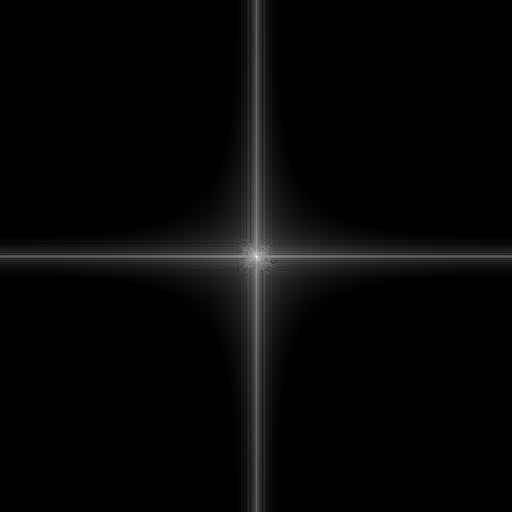
\includegraphics[width=0.22\linewidth]{img/ch5/3-fft.png}
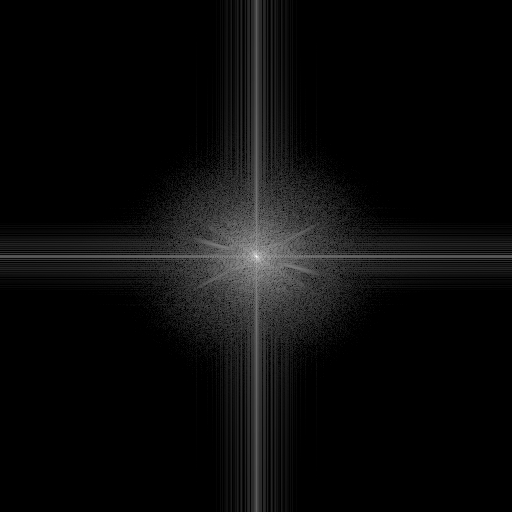
\includegraphics[width=0.22\linewidth]{img/ch5/5-fft.png}
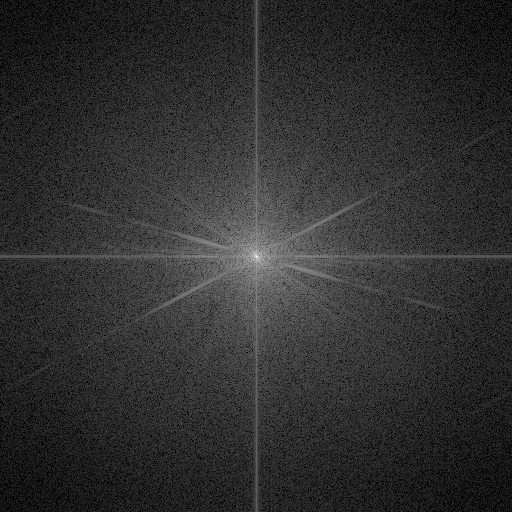
\includegraphics[width=0.22\linewidth]{img/ch5/7-fft.png}
\caption{Cameraman: reconstructed multiresolution levels 1, 3, 5, and 7, along with their corresponding Fourier spectra.}
\label{f:lod}
\end{figure}

The training times for each stage of the network were as follows: 5s, 4s, 3s, 11s, 17s, 29s, and 48s, with a total training time of 117s. These times were measured on a Windows 10 laptop with an NVIDIA RTX A5000 Laptop GPU. The variability in training time reflects the adaptive training regime and the different sample sizes at each level of the Gaussian pyramid.

% The training evolution is depicted in the graph of Figure \ref{f:training-epochs} that shows the convergence of the MSE loss with the number of epochs for each multiresolution levels 1, 3, 5, and 7. It is worth pointing out the qualitative behavior of the network, in that the base level (stage 1) takes more than 200 epochs to reach the limit, while detail levels (stages 3, 5, 7) take less than 150 epochs to converge.  It is like, there are two different modes, one to fit the base level and the other for the detail levels.

Figure~\ref{f:training-epochs} shows the training evolution for stages 1, 3, 5, and 7, plotting MSE loss against the number of epochs. Notably, the network exhibits two distinct convergence behaviors: the base stage (level 1) requires more than 200 epochs to converge, while the higher-resolution stages (levels 3, 5, and 7) converge in fewer than 150 epochs. This is consistent with the intuition that the base level captures coarse details, while subsequent stages focus on refining finer details.

\begin{figure}[!h]
\centering
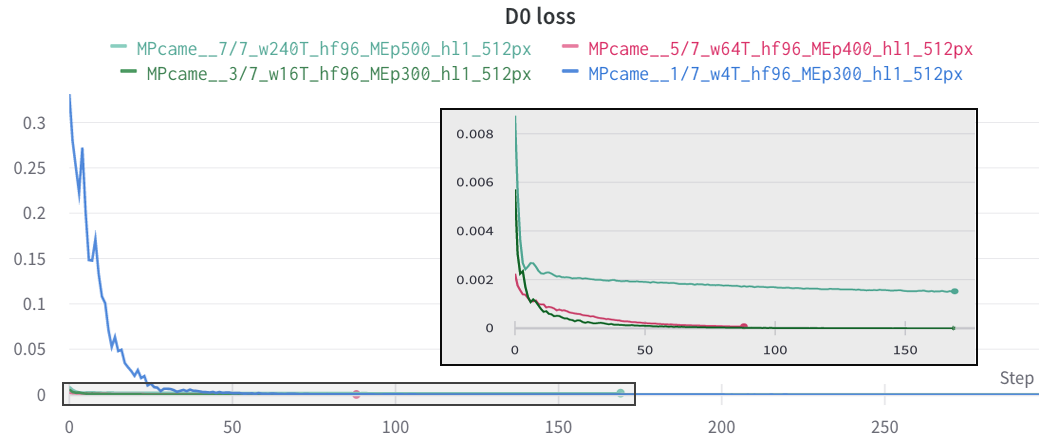
\includegraphics[width=\linewidth]{img/ch5/stages-training-epochs.png}
\caption{Training convergence behavior for the "Cameraman" image at multiresolution levels 1, 3, 5, and 7 (Fig.~\ref{f:lod}).}
\label{f:training-epochs}
\end{figure}


Finally, inference times for reconstructing the image range from 0.02 seconds on the GPU to 0.7 seconds on the CPU, making the network fast enough for interactive visualization tasks.

\subsection{Texture}

In this second example, we apply the MR-Net architecture to model texture and visual patterns, which are central in many image-based applications ranging from photorealistic simulations to interactive gaming. Currently, more and more image rendering relies on some kind of graphics acceleration, including GPUs integrated with neural engines. In that context, compact and efficient neural image representations that support levels of detail may be a valuable resource.

For this experiment, we use an image of a woven fabric, which features distinct patterns that test the MR-Net's ability to capture intricate visual details across different resolutions. The original image has a resolution of \(1025 \times 1025\) pixels, and the MR-Net model operates with 5 levels of detail. Figure~\ref{f:pattern} presents our experimental results. Figure~\ref{f:pattern}(B) shows the image in the original resolution, while Figures~\ref{f:pattern}(A) and (C) show zoomed-in and zoomed-out views respectively.

\begin{figure}[!h]
\centering
\begin{subfigure}{0.39\linewidth}
  \centering
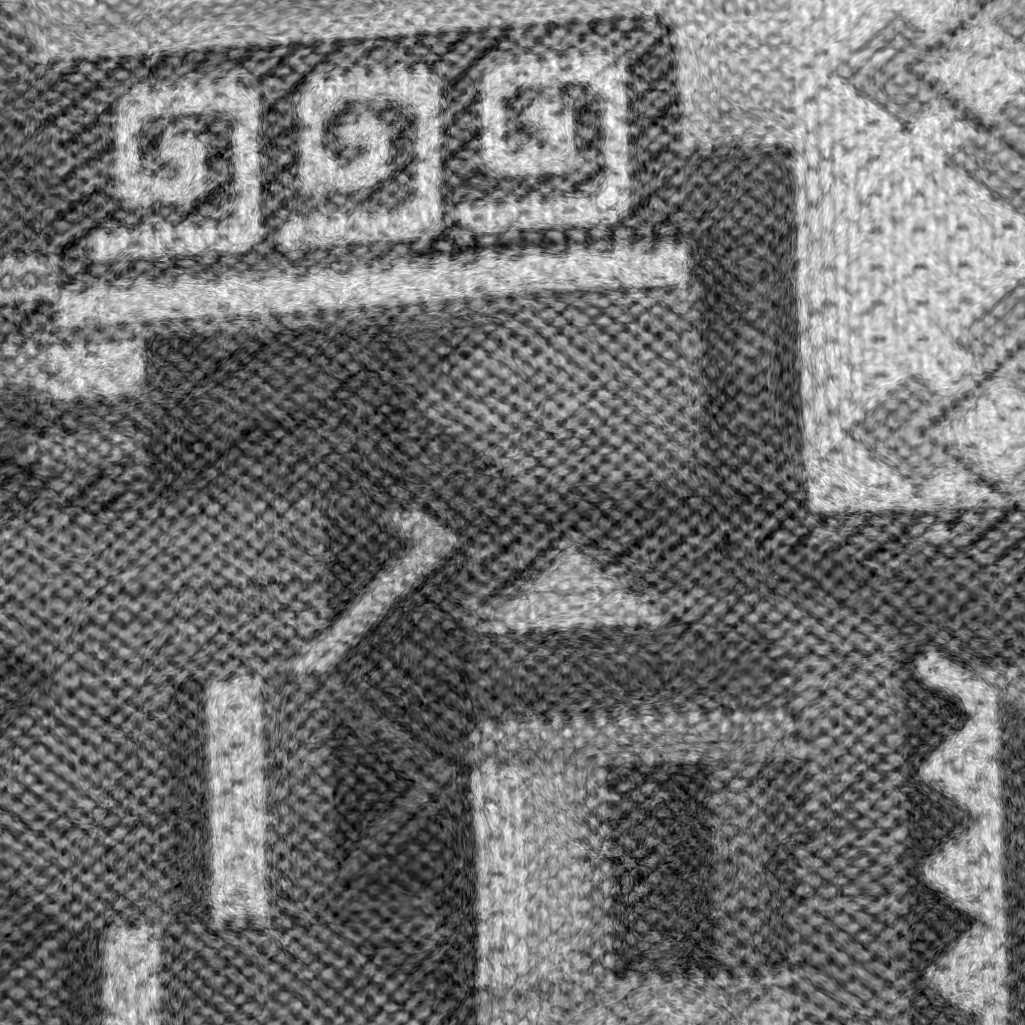
\includegraphics[width=\linewidth]{img/ch5/tex_zoom_in_stage_5.png}
\caption{}
\label{f:patternA}
\end{subfigure}
\begin{subfigure}{0.39\linewidth}
  \centering
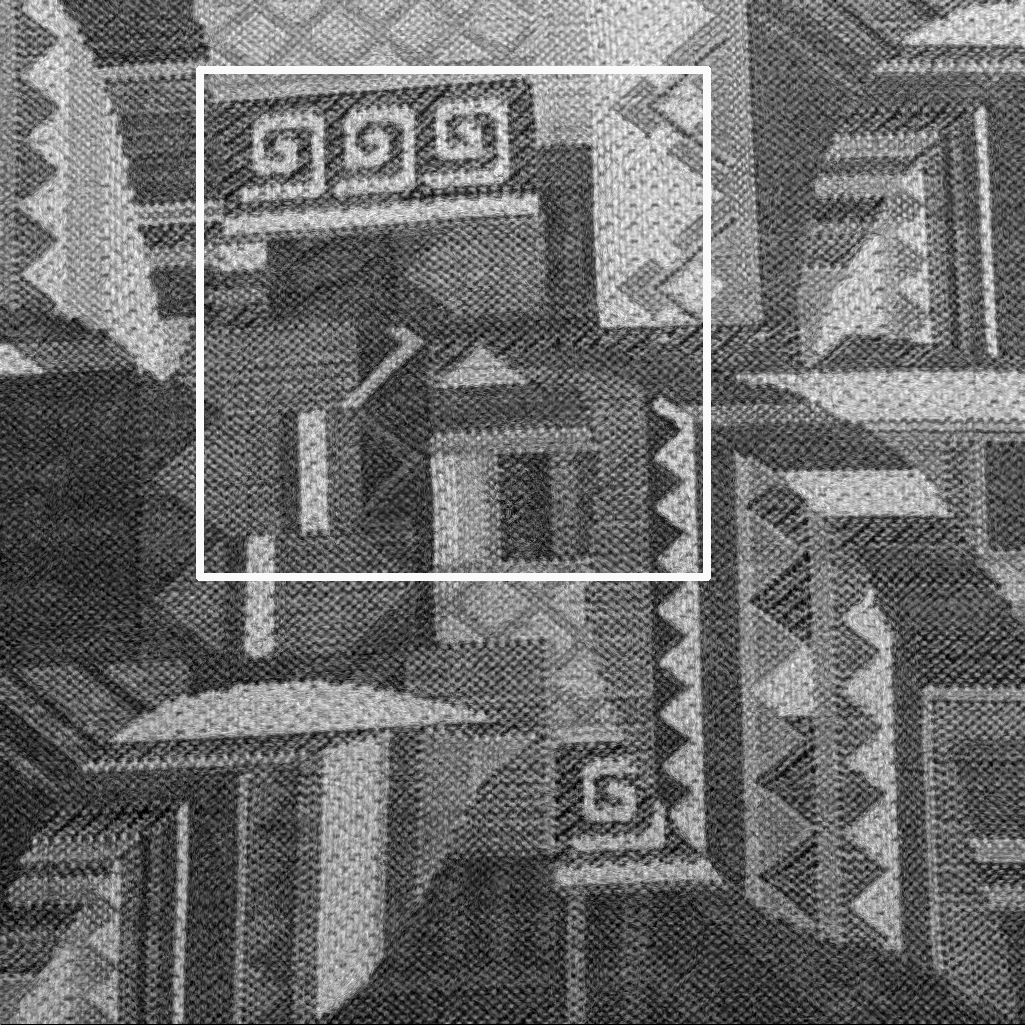
\includegraphics[width=\linewidth]{img/ch5/tex_stage_5.png}
\caption{}
\end{subfigure}
\begin{subfigure}{.19\linewidth}
  \centering
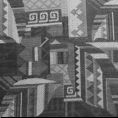
\includegraphics[width=\linewidth]{img/ch5/tex_zoom_out_stage_3.png}\\
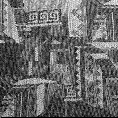
\includegraphics[width=\linewidth]{img/ch5/tex_zoom_out_stage_5.png}
\caption{}
\label{f:patternC}
\end{subfigure}
\caption{Woven Fabric Texture: (A) zoomed-in view; (B) original resolution; (C) zoomed-out views.}
\label{f:pattern}
\end{figure}


In Figure \ref{f:patternA}, we zoom into a detail at \(562 \times 562\) pixels, marked by a white rectangle in panel (b), creating a zoom factor of approximately 1.8 times; then, we scale it up to \(1025 \times 1025\). The zoomed-in region extrapolates fine details, which remain visually coherent at this higher resolution, demonstrating the model's capacity for fine-detail extrapolation.

In contrast, Figure \ref{f:patternC} shows a zoom-out to \(118 \times 118\) pixels, enlarged to \(501 \times 501\) pixels for visualization purposes. The top sub-image depicts the MR-Net reconstruction at the appropriate level of detail (\red{approximately 0.92}), while the bottom sub-image shows a simple point-sampled nearest neighbor reduction. Notice that the MR-Net reconstruction preserves smooth transitions and avoids aliasing, while the point-sampled image displays visible aliasing artifacts.

These two behaviors in the experiment, \textit{magnification} (zoom-in) and \textit{minification} (zoom-out), are classical resampling regimes used in image processing \citep{pixel} and computer graphics. Magnification requires pixel interpolation, whereas minification requires pixel integration over an area. MR-Net handles both operations automatically. Note that we chose fractional scaling factors in both cases to demonstrate the continuous properties in space and scale of our model.

\subsection{Anti-aliasing}

In the previous subsection, we demonstrated how the level of detail mechanism in MR-Net enables alias-free rendering for zooming operations. In that case, a uniform LOD was sufficient across the image due to the nature of 2D zooming. However, in more complex scenarios, such as texture mapping onto 3D surfaces, the level of detail must vary spatially depending on the distance from the camera to the surface. This presents a challenge, as the level of detail needs to adapt to the projective transformations that introduce foreshortening.

We now illustrate how MR-Net handles this challenge through a simple anti-aliasing example. Let \(I\) be a checkerboard image, and \(T\) be a homography mapping pixel coordinates \(x = (x_1, x_2)\) on the screen to texture coordinates \(u = (u_1, u_2)\) on \(I\). Let \(f: \mathbb{R}^2 \times [0, N] \to \mathbb{R}\) represent an MR-Net with \(N\) stages, approximating a multiresolution representation of \(I\).

In Figure \ref{fig:alias-naive-checkerboard}, we observe aliasing artifacts caused by applying the inverse of \(T\) to the checkerboard pattern without multiresolution control. This results in noticeable high-frequency noise, especially at larger distances from the camera. In contrast, Figure \ref{fig:antialias-mnet-checkerboard} shows the result using MR-Net's multiresolution model, which eliminates the aliasing artifacts and produces a smooth, anti-aliased rendering.

% \begin{figure}[!h]
% \centering
% 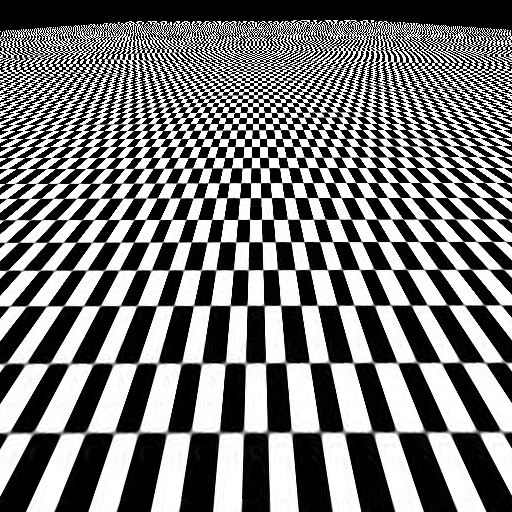
\includegraphics[width=0.46\linewidth]{img/ch5/im_0_alias.png}
% 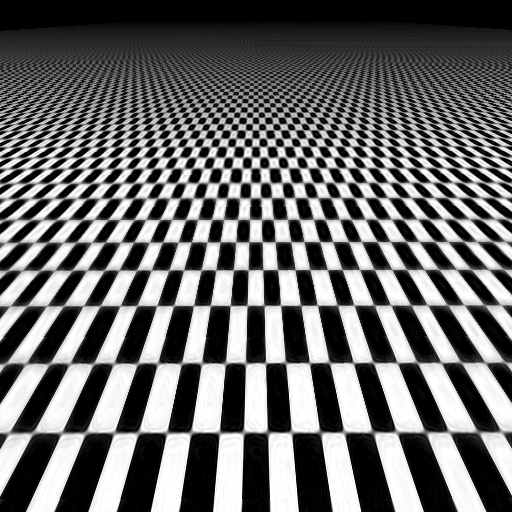
\includegraphics[width=0.46\linewidth]{img/ch5/im_0_anti_alias.png}
% \centerline{(a)\hfil\hfil(b)}
% \caption{Checkerboard in perspective: (A) aliasing from point sampling; (B) M-Net anti-aliased reconstruction.}
% \label{f:alias}
% \end{figure}

\begin{figure}[!h]
  \centering
  \begin{subfigure}{0.46\linewidth}
    \centering
  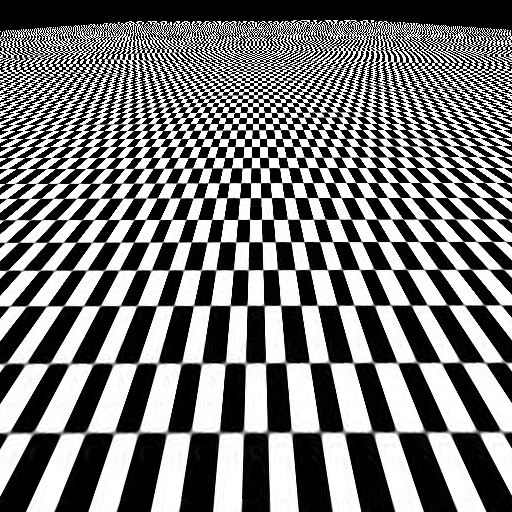
\includegraphics[width=\linewidth]{img/ch5/im_0_alias.png}
  \caption{}
  \label{fig:alias-naive-checkerboard}
  \end{subfigure}
  \begin{subfigure}{0.46\linewidth}
    \centering
  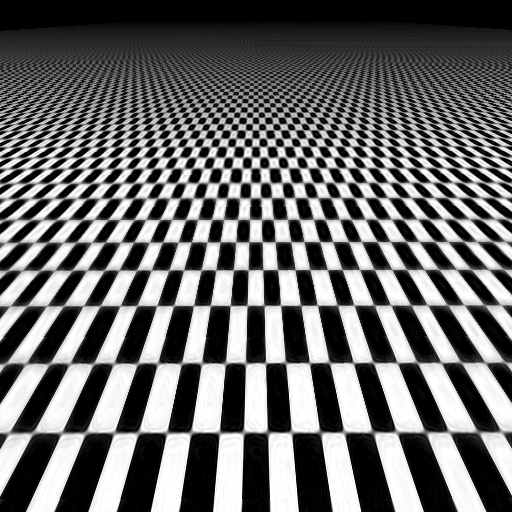
\includegraphics[width=\linewidth]{img/ch5/im_0_anti_alias.png}
  \caption{}
  \label{fig:antialias-mnet-checkerboard}
  \end{subfigure}
  \caption{Checkerboard in perspective: (A) aliasing from point sampling; (B) M-Net anti-aliased reconstruction.}
  \label{f:alias-checkerboard}
\end{figure}


The anti-aliasing effect is achieved by selecting the appropriate level of detail using the scale parameter \(\lambda(x)\), as defined by Heckbert's formula for texture mapping~\citep{heckbert1983texture}:

% The above procedure reduces aliasing at large distances. Specifically,
% we define the scale parameter $\lambda(x)$ for $f$ at a pixel $x$ using the Heckbert 's formula~\cite{heckbert1983texture}:

\begin{align}
    \lambda(x)=\max\left\{\sqrt{\left(\frac{\partial u_1}{\partial x_1}\right)^2+\left(\frac{\partial u_2}{\partial x_1}\right)^2}, \sqrt{\left(\frac{\partial u_1}{\partial x_2}\right)^2+\left(\frac{\partial u_2}{\partial x_2}\right)^2}\right\}.
\end{align}

% Thus $\lambda(x)$ is the bigger length of the parallelogram generated by the vectors $\frac{\partial T}{\partial x_1}$ and $\frac{\partial T}{\partial x_2}$. 
% We scale $\lambda$ such that $\lambda\big([-1,1]^2\big)\subset[0,N]$.
% Thus, $f(x,\lambda(x))$ is the desired level of detail $\lambda(x)$ of $f$.

Here, \(\lambda(x)\) represents the maximum length of the parallelogram generated by the Jacobian vectors \(\frac{\partial T}{\partial x_1}\) and \(\frac{\partial T}{\partial x_2}\). By normalizing \(\lambda(x)\) to fit within the range \([0, N]\), the desired level of detail at each pixel is determined. Thus, the MR-Net output \(f(x, \lambda(x))\) provides a continuous and spatially adaptive level of detail that mitigates aliasing caused by projective transformations.

\section{Comparisons}
\label{sec:comparison}

In this section, we compare the performance of MR-Net with two other notable methods for neural image representation: SIREN \citep{sitzmann2019siren} and BACON \citep{bacon2021}. The evaluation focuses on three key aspects: (i) the quality of image fitting, (ii) the model size, and (iii) the frequency spectra of reconstructions at different levels of detail. In a broader quantitative evaluation using the "Kodak Lossless True Color Image Suite" \citep{KodakDataset}, we assess metrics such as Peak Signal-to-Noise Ratio (PSNR), model size, and training time for various configurations.

\subsection{Image Fitting Evaluation}

We first evaluate each model's performance in fitting a single image, using the "Cameraman" image as a reference. For a fair comparison with SIREN, which is not designed for multiresolution data, we only evaluate the PSNR of the final image at its highest resolution, which is $512 \times 512$. Table~\ref{t:comp} summarizes the results.

\begin{table}[!h]
\centering
\small
\begin{tabular}{|l|r|r|r|}
\hline
Model & \# Params $(\downarrow)$ & PSNR $(\uparrow)$ & \# Levels \\
\hline
SIREN~\cite{sitzmann2019siren} & 198K & {\bf 34.1} dB & 1  \\
BACON~\cite{bacon2021} & 398K & 33.1 dB & 7 \\
MR-Net (Ours) & {\bf 196K} & 33.8 dB & 7  \\
\hline
\end{tabular}
\caption{Comparison of SIREN, BACON, and MR-Net on image fitting.}
\label{t:comp}
\end{table}

The M-Net parameters are: 1 hidden layer per stage; 96 hidden features per layer in the first 6 stages, and 256 hidden features in the last stage; $\omega \in [4, 256]$ and trained with a Gaussian Pyramid of 7 levels. The model size has 195648 parameters and the PSNR of the final image reconstruction is 33.8~dB. The model was trained for 300 epochs per stage.

SIREN's configuration is based on the authors' original experiments, utilizing 3 hidden layers with 256 units each, and $\omega_0 = 30$. This model comprises 198K parameters and is trained for 2000 epochs, achieving a PSNR of 34.1 dB. Although SIREN performs slightly better in terms of PSNR, the M-Net achieves comparable results while encoding 7 levels of detail in the same model. Figure~\ref{f:siren} shows a comparison between our M-Net and SIREN. Notice that, although M-Net presents a PSNR close to Siren's in this example, visually, it seems that it can better represent high frequency details.

\begin{figure}[!h]
  \centering
  \begin{subfigure}{0.45\linewidth}
    \centering
  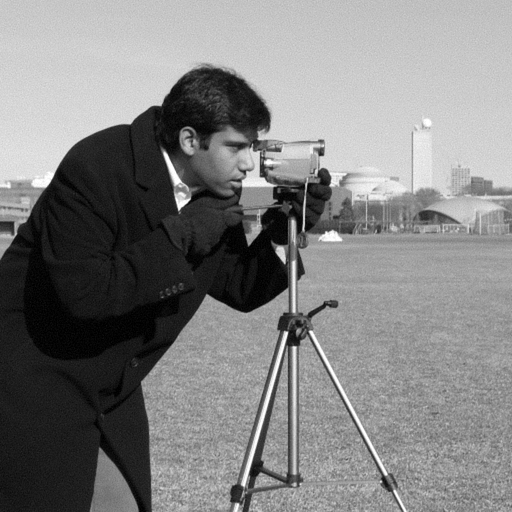
\includegraphics[width=\linewidth]{img/ch5/rec-MR-Net.png}
  \caption{M-Net}
  \end{subfigure}
  \begin{subfigure}{0.45\linewidth}
    \centering
  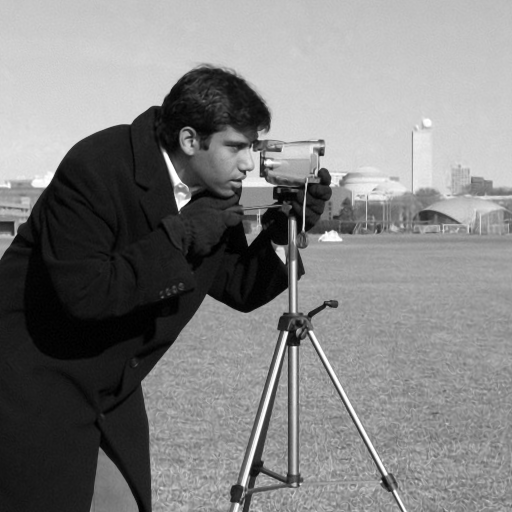
\includegraphics[width=\linewidth]{img/ch5/rec-SIREN.png}
  \caption{SIREN}
  \end{subfigure}
  \caption{Comparison of image reconstructions for M-Net and SIREN.}
  \label{f:siren}
\end{figure}


For BACON we also based the configuration on their paper examples and code released by the authors, keeping 256 hidden features. However, we adjusted the number of hidden layers to 6 for it to output 7 levels of details as the M-Net in this setting. Accordingly, the total number of parameters is 398343. The PSNR of the original image level is 33.1 db.

On this experiment, MR-Net outperforms BACON in terms of model size, achieving nearly 50\% fewer parameters while maintaining comparable PSNR. Compared to SIREN, MR-Net offers similar PSNR but with the advantage of multiresolution capabilities in a model of comparable size. The visual quality of MR-Net's reconstructions also appears sharper, particularly for finer details.

\subsection{Frequency Spectra Evaluation}
\label{sub:spectra-eval}

Next, we analyze the frequency spectra of the image reconstructions produced by BACON and MR-Net at different levels of detail.

Figures~\ref{f:bacon} and~\ref{f:mnet} show both the reconstructed images and their corresponding frequency spectra for three levels of detail in the BACON and M-Net models, respectively (1, 2, 6) and (3, 5, 7). Note that, as Bacon is not trained with multiresolution data, we select these levels to better match the frequency spectra between the representations.

\begin{figure}[!h]
\centering
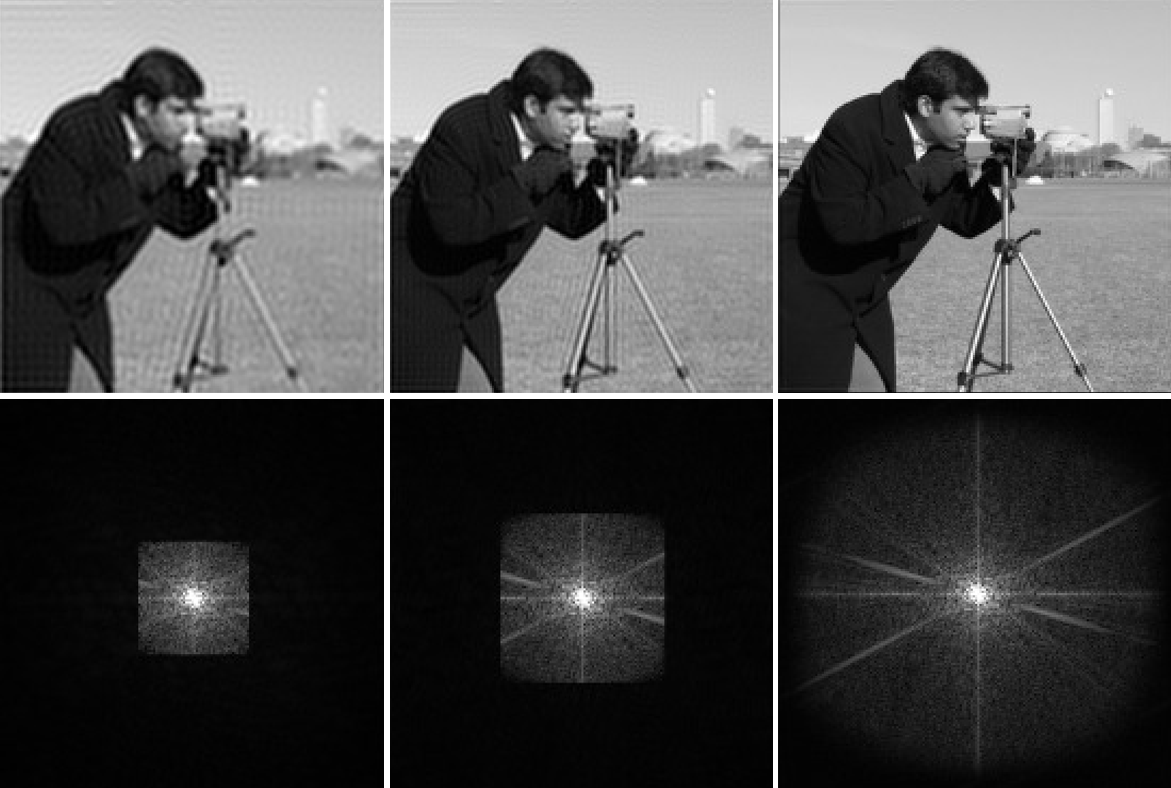
\includegraphics[width=0.85\linewidth]{img/ch5/bacon-3.png}
\centerline{\small Level 1 \hfil Level 2 \hfil Level 6}
\caption{BACON image reconstructions and corresponding frequency spectra at different levels.}
\label{f:bacon}
\end{figure}

\begin{figure}[!h]
\centering
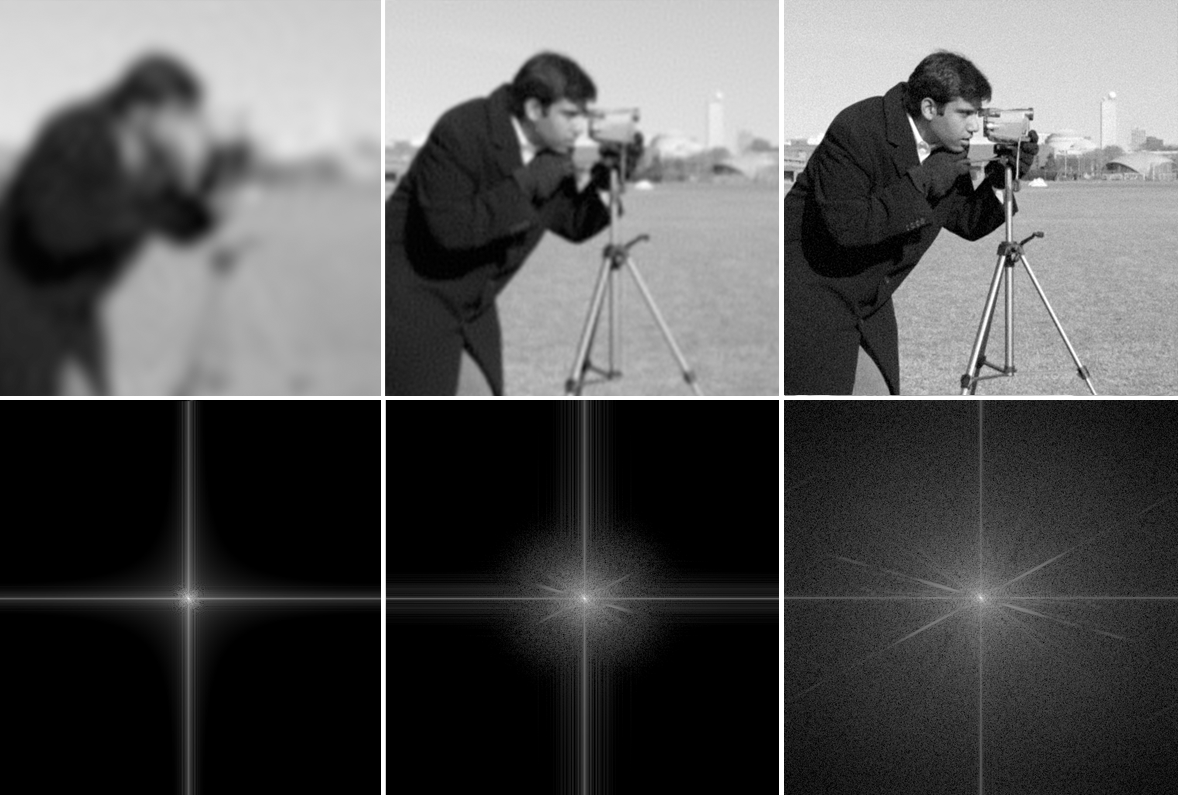
\includegraphics[width=0.85\linewidth]{img/ch5/m-net-3.png}
\centerline{\small Level 3 \hfil Level 5 \hfil Level 7}
\caption{MR-Net image reconstructions and corresponding frequency spectra at different levels.}
\label{f:mnet}
\end{figure}


BACON controls the frequency band for level of detail by truncating the signal's spectrum. Figure~\ref{f:bacon} shows that the center of the spectrum images of Levels 1, 2, 6 are all similar. This is analogous to applying a low-pass filter with non-ideal shape in the frequency domain, which results in an image with ringing effect (see the silhouettes propagating all over Figure~\ref{f:bacon} (left)). In contrast, MR-Net frequency spectra more closely resemble the expected result of applying Gaussian filters to high-resolution images in a multiresolution framework. Figure~\ref{f:mnet} shows that MR-Net achieves smoother transitions between levels, maintaining better control over the frequencies captured at each stage.



\subsection{Kodak Dataset Evaluation}\label{sub:kodak}

% The ``Kodak Lossless True Color Image Suite" is a set of 24 images, originally $768 \times 512$ in size, that were extensively used in the image processing literature. For each image, we center crop a square of $512\times 512$ pixels, convert it to grayscale and evaluate the PSNR, model size and training time using different network configurations of each model. The average results over this dataset are summarized in Table~\ref{t:kodak}. 

We further evaluate MR-Net, SIREN, and BACON on the "Kodak Lossless True Color Image Suite," which consists of 24 images, each of size $768 \times 512$. For each image, we center-crop a $512 \times 512$ region, convert it to grayscale, and compute the PSNR, model size, and training time for various configurations. The average results are presented in Table~\ref{tab:kodak}.

We present the training time in a relative scale. All models were trained in a NVidia GeForce RTX 3080 with 10GB of GPU memory. The longest average running time observed was 40 minutes and 33 seconds (2433 seconds) when training an instance of BACON with 6 hidden layers and 256 neurons per layer (Bacon\_6hl\_256). Therefore, we display this row as 100\% and all others as a fraction of it.


\begin{table}[!h]
\centering
\small
\begin{tabular}{|l|r|r|r|}
\hline
Model                    & \# Params $(\downarrow)$ & PSNR $(\uparrow)$ & Time $(\downarrow)$ \\
\hline
SIREN$_\text{3hl\_256hf}$        & 198K      & 41.93    & 8.7\%       \\
SIREN$_\text{4hl\_256hf}$        & 264K      & 44.63    & 11.0\%      \\
SIREN$_\text{5hl\_256hf}$        & 330K      & 46.25    & 13.6\%      \\
SIREN$_\text{3hl\_512hf}$        & 790K      & 48.57    & 23.8\%      \\
\hline
BACON$_\text{5hl\_128hf}$        & 84K       & 27.42    & 36.2\%      \\
BACON$_\text{6hl\_128hf}$        & 101K      & 28.23    & 44.1\%      \\
BACON$_\text{4hl\_256hf}$        & 266K      & 33.69    & 60.8\%      \\
BACON$_\text{5hl\_256hf}$        & 332K      & 34.13    & 75.7\%      \\
BACON$_\text{6hl\_256hf}$        & 398K      & 34.31    & 100.0\%     \\
\hline
% MNet$_\text{5hl\_96hf}$          & 85K       & XXXX    & 5.4\%       \\
% MNet$_\text{6hl\_96hf}$          & 104K      & XXXX    & 6.7\%       \\
% MNet$_\text{7hl\_96hf}$          & 123K      & XXXX    & XXX\%       \\
MNetCap$_\text{2stg\_256hf}$    & 117K      & 35.14    & 3.4\%       \\
MNet$_\text{7stg\_24\_256hf}$          & 193K      & 38.42    & 9.3\%       \\
MNet$_\text{7stg\_96\_256hf}$          & 196K      & 35.04    & 9.6\%       \\
MNet$_\text{6stg\_24\_288hf}$          & 197K      & 40.85    & 8.2\%       \\
MNetCap$_\text{128\_192\_256}$ & 195K      & 41.05    & 8.0\%       \\
MNetCap$_\text{3stg\_256hf}$           & 332K      & 45.46    & 11.4\%     \\
\hline
\end{tabular}
\caption{\label{tab:kodak} Comparisons on Kodak Lossless True Color Image Suite. We present the training time relative to BACON$_\text{6hl\_256hf}$ which took 2433 seconds to train.}
\label{t:kodak}
\end{table}


We evaluate four different instances of SIREN: three with 3, 4, and 5 hidden layers, each containing 256 neurons per layer, and a fourth with 3 hidden layers, each having 512 neurons. For BACON, we examine five configurations: models with 5 and 6 hidden layers containing 128 neurons per layer, and models with 4, 5, and 6 hidden layers, each with 256 neurons per layer.

All M-Net stages have depth $2$, so we vary the number of stages and their width. Since our focus is on evaluating reconstruction at the final resolution level, we compare M-Net with and without multiresolution data. Notice that we have more flexibility on the M-Net configuration as each MR-Module can have a different size. We decided to explore a few configurations with heterogeneous stages, choosing smaller modules for the coarsest levels, and bigger modules for the finest ones.

When training with a Gaussian pyramid, we evaluate the following configurations: MNet$_\text{7stg\_96\_256hf}$, which consists of 7 stages with widths [96, 96, 96, 96, 96, 96, 256]; MNet$_\text{7stg\_24\_256hf}$, with 7 stages and widths [24, 32, 64, 96, 96, 160, 256]; and MNet$_\text{6stg\_24\_288hf}$, with 6 stages and widths [24, 32, 64, 96, 160, 288]. Despite the different architectures, these models have about the same number of total parameters. When training capacity based instances using only the original image, we evaluate: MNetCap$_\text{2stg\_256hf}$  with 2 stages and width $256$; MNetCap$_\text{2stg\_256hf}$, with 2 stages and width 256; MNetCap$_\text{3stg\_256hf}$, with 3 stages and width 256; and MNetCap$_\text{128\_192\_256}$, with 3 stages of increasing width (128, 192, 256).

Within each model category, we observe a general trend: increasing the total number of parameters tends to improve reconstruction quality. For instance, SIREN and M-Net models of comparable size yield similar PSNR values, whereas BACON consistently underperforms relative to the other two in terms of PSNR at the final resolution. The exception occurs when we compare the M-Net models MNet$_\text{7stg\_24\_256hf}$ and MNet$_\text{7stg\_96\_256hf}$. Despite both having 7 stages, the former, which distributes capacity unevenly across stages, performs better. This heterogeneous configuration allocates fewer parameters to the coarser levels, which primarily encode low-frequency information, allowing more capacity to be dedicated to the finer levels where high-frequency details are essential. 

The advantage of this heterogeneous distribution is further demonstrated when comparing MNet$_\text{7stg\_24\_256hf}$ and MNet$_\text{6stg\_24\_288hf}$. By reducing the number of stages and increasing the width of the finest stages to maintain a similar model size, the latter model achieves better performance, reinforcing the idea that finer stages benefit from additional capacity.


Each M-Net model is trained for 2000 epochs per stage, while the others are trained for 5000 epochs. Although we train M-Net for more epochs, notice that due to our scheduled training scheme, we only update the parameters of a single stage each 2000 epochs. Besides that, when training with multiresolution data, the coarsest stages are trained with fewer samples. This scheduling helps the M-Net models to train more quickly than their counterparts, even with a larger number of parameters or epochs. 

For example, training MNet$_\text{6stg\_24\_288hf}$, with 197,182 parameters, takes 199 seconds for 12,000 epochs, which is comparable to the 211 seconds needed to train a SIREN model with 3 hidden layers and 198,401 parameters for 5000 epochs. Both are significantly faster than training a BACON model with fewer parameters (BACON$_\text{5hl\_128hf}$ takes 881 seconds). The highest quality M-Net model in this evaluation, a M-Net capacity based with 331523 parameters and 3 levels of details (MNetCap$_\text{3stg\_256hf}$), completes training in 278 seconds for 6000 epochs, which is only 15\% of the time required to train a BACON model of the same size (BACON$_\text{5hl\_256hf}$ takes 1842 seconds). Moreover, this M-Net model's training time is comparable to that of a smaller SIREN model (SIREN$_\text{4hl\_256hf}$ with 264,001 parameters) trained for 5000 epochs, which takes 267 seconds.

We conclude that M-Net offers not only competitive PSNR values but also significantly reduced training times compared to BACON, and in many cases, even outperforms SIREN in terms of training efficiency. This balance between model complexity, reconstruction quality, and training speed makes M-Net a highly practical solution for image reconstruction tasks, particularly when multiresolution capabilities are essential.

\section{Considerations for Other MR-Net subclasses}\label{sec:considerations}

Up until now, we have focused exclusively on the M-Net subclass. In this section, we expand the discussion to include a brief comparison between M-Net and the other MR-Net subclasses, namely S-Net and L-Net.

For S-Net, we define a configuration composed of 3 stages, with 1000, 2000, and 4000 hidden features per layer respectively, resulting in a total of $28000$ parameters. For the L-Net, we use 3 stages, each with 2 hidden layers containing 40, 60, and 80 neurons for each layer. This L-Net version has a total of $24280$ parameters. Finally, for the M-Net, we set 3 stages with 1 hidden layer each, contatining 30, 40, and 80 hidden features per layer, respectively, resulting in $23100$ parameters. 

The training regimen for these models was adapted to their architectural characteristics: S-Net was trained for a maximum of 4000 epochs, while both L-Net and M-Net were trained for up to 2000 epochs. All models were evaluated on a set of 10 images with a resolution of $128 \times 128$. As we can see in Table \ref{t:comp-variants}, on average, considering the PSNR, the M-Net outperforms the other variants when reconstructing images.

\begin{table}[!h]
  \centering
  \small
  \begin{tabular}{|l|r|r|r|}
  \hline
  Model & \# Params $(\downarrow)$ & PSNR $(\uparrow)$  \\
  \hline
  S-Net & 28000 & 42.1 dB  \\
  L-Net & 24280 & 47.8 dB \\
  M-Net & {\bf 23100} & {\bf 51.1} dB   \\
  \hline
  \end{tabular}
  \caption{Comparison of MR-Net subclasses in terms of parameters and PSNR.}
  \label{t:comp-variants}
\end{table}

Nonetheless, here it is appropriate to make a few considerations about the S-Net and L-Net variants. The S-Net represents the image as a weighted sum of sine functions. In that sense, S-Net is equivalent to BACON and other Multiplicative Filter Networks based on sinusoidal atoms, providing a more straighforward control over the frequencies represented. Figure \ref{f:albert-snet} presents the gradient magnitude and frequency spectra from an image predicted by S-net, where it has three stages.


\begin{figure}[!h]
\centering
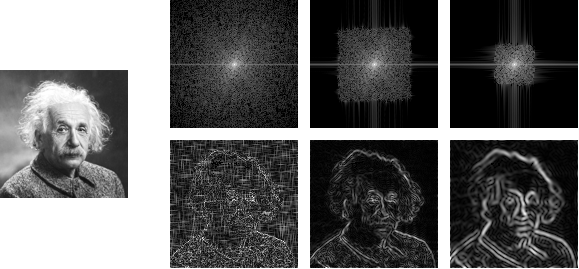
\includegraphics[width=0.8\linewidth]{img/ch5/albert.png}
\caption{S-Net Gradient Magnitude and frequency spectra.}
\label{f:albert-snet}
\end{figure}


L-Net's representation is inspired by level-of-detail techniques, where each stage is handled by independent MR-Modules. This design makes L-Net particularly well-suited for image processing tasks that involve operations in the gradient domain, akin to methods based on Laplacian pyramids. The capacity to decompose the image into finer details at different stages allows L-Net to capture both low and high-frequency components effectively, offering a hierarchical reconstruction approach. Figure \ref{f:albert-lnet} displays the L-Net reconstruction of the same image used for S-Net and shows the frequency spectra for each of L-Net's stages.

\begin{figure}[!h]
\centering
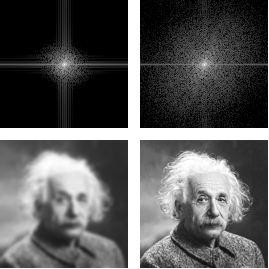
\includegraphics[width=0.80\linewidth]{img/ch5/albert-lnet.png}
\caption{L-Net reconstruction and frequency spectra.}
\label{f:albert-lnet}
\end{figure}



%TO DO REWRITE EXPERIMENTS S-NET, L-NET, M-NET

%We intend to study and compare the three variants of the MR-Net architecture and also to develop imaging applications in dir,ections pointed out above for L-Net, complementing the ones we have presented in the paper for M-Net.

\section{Limitations}

One key challenge we identified is the importance of selecting appropriate values for the $\omega$ parameter, which defines the spatial frequency of the first sinusoidal layer for each MR-Module of the network. The choice of $\omega$ significantly impacts the model's ability to reconstruct fine details, and may also introduce noise if it is too high.

In the case of pure sine MR-Modules like S-Net, the Nyquist frequency serves as a reliable reference point for determining frequency intervals at each stage, ensuring that the model captures all relevant frequencies without introducing aliasing. However, for deeper networks such as M-Net, the situation is more complex. M-Net can learn higher frequencies during training, even those that were not explicitly introduced at initialization. This emergent behavior, while beneficial, introduces uncertainty, as it becomes harder to predict the exact frequency range the model will cover after training.

% In our experiments, we have determined the $\omega$ values for initialization of the frequency bands empirically, testing values below the Nyquist frequency as described in Sec \ref{s-frequency-initialization}. To better harness the power of sinusoidal neural networks, it is important to develop mathematical theories to understand how the composition of sine functions introduces new frequencies based on the initialization of the network. In future works we intend to investigate the use of the results in \cite{novello2022understanding} to compute or bound these~frequencies.

In our experiments, we determined the $\omega$ values for the initialization of the frequency bands empirically, as discussed in Section \ref{sec:frequency-initialization}. We experimented with values below the Nyquist frequency, aiming to strike a balance between capturing enough detail and avoiding overfitting to high-frequency noise. However, this empirical approach has its limitations. Without a formal framework to guide the initialization process, selecting $\omega$ can become a trial-and-error procedure that might not generalize well across different datasets or tasks.

To fully leverage the capabilities of sinusoidal neural networks, future work should focus on developing a more rigorous mathematical understanding of how sine function compositions introduce new frequencies as the network trains. A promising direction for this is to build on the theoretical results in \cite{novello2022understanding}, which provide insights into how the composition of sine functions generates higher-order frequencies. Incorporating these results could lead to methods for calculating or bounding the frequencies learned by the network, providing more control over the model's frequency response.

Moreover, the sinusoidal neural networks we have been exploring are closely related to the Fourier transform, which provides an analytical interpretation of a signal in terms of its frequency components. However, this interpretation does not constitute a representation in the formal sense used in \textit{representation theory}. In contrast, the Fourier series offers a true representation for periodic functions by expressing them as a sum of Fourier basis functions. Restricting the function space that our networks can learn to this structured representation could offer new insights and advantages, which we will explore in detail in the next chapter.